%avoid page number on blank pages when cleared
\thispagestyle{empty}
\cleardoublepage  
\chapter{Methodology}
\label{chap:methodology}

\section{Solution Methodology Design}
\label{sec:solmet}

This sections presents the solution methodology which consists in the different
steps in image processing that must be performed in order to successfully fit the shape of 
\emph{C.elegans} worms present in digital images. First a general description
of the solution is presented where the shape fitting approach is explained, indicating
the different processes involved in the solution design. Then for each process 
a reasoning of its requirement and usefulness is given, as well as 
the corresponding 
implementation approach.

\subsection{Previous reasoning}
\label{sec:reasoning}

As stated in \cite{binaryshape} and also covered in
\cite{deformable,matching2,matchingbook} shape 
matching is usually accomplished adopting a shape
descriptor and then placing a constructed shape sufficiently 
close to the image shape and adjusting the values of 
the parameters of the descriptor until a match is found.
A shape descriptor is a representation of a 
specific class of objects that is defined in geometrical
terms. It is comprised of a number of parameters, where 
different values for each parameter give different 
shapes of a given class of objects.
This approach is appropriate when the objects
that are to be matched can be categorized in a certain 
class and thus can be represented or described in terms
of geometry, \emph{i.e.} a shape descriptor.\\

The problem of study aims the detection of worms,
particularly those belonging to the \emph{C.elegans} species. Given
the vermiform (worm shape) property of these individuals,
the objects to detect can be defined as part of a 
\emph{worm} class,
that would refer geometrically to long, thin and cylindrical 
shapes, in 
general terms. Following this idea, a shape descriptor could be
designed that comprehends a cylindrical, long and connected
shape, with two endpoints and different thickness along a medial
axis. Then the problem would be reduced to find every pair of
endpoints belonging to each worm in the image, place an approximated
shape (built through the shape descriptor) near the matching worm,
and adjust the values of the parameters of the shape descriptor until
an acceptable match is found.\\

To design a methodology for the solution of the problem the following
points must be taken into consideration: the nature of the input
images, the positional identification of worms in the global image,
the gathering and loss of information and the efficacy and efficiency
of each of the involved processes (and their respective algorithms).
For this study the input images consist of a number of worms that
are put together in liquid media. The image can contain some noise such as
shadows, water bubbles or little remains that do not belong to the worms, so
these last, as objects of study, must be separated from the rest of 
the information in the image. The position of each individual
worm in the image is variable and can be distinguished into two 
groups: \emph{worm clusters} and \emph{isolated worms}. A 
\emph{worm cluster} corresponds to a group of worms in which 
each worm is connected to any other directly or indirectly
through overlapping. It can also be described as a group of worms in which a 
path can be traced from every worm to another without passing over 
background pixels. On the other hand, an \emph{isolated worm} is such
that it is surrounded by background pixels and does not overlap
with any other worm. The image can be segmented by separating the different 
\emph{worm clusters} and \emph{isolated worms}, so each segment
can be processed individually. The contour of \emph{isolated worms} can be
traced automatically following the pixels that are closest to background pixels.
These can also be used to generate a profile that will set the general values
for the shape descriptor that best represents the shape of the worms in the image.
The worms that are clustered can be matched through an energy minimization
process, based on the manipulation of the shape descriptor and its distance
to the matching image, in order to obtain the best possible match.

\subsection{Methodology description}
\label{met:description}

Following the previous reasoning, a methodology was designed taking into account
the main components of the matching process, as reasoned before, such as: 
determination of the objects 
of study, objects segmentation, worm shape descriptor and matching based on 
energy minimization.
Below the solution methodology is described, pointing out the sequential steps
that are followed to match and fit the shape of every worm in the input image.
In Fig. \ref{fig:methsol}, a graphical description of the solution methodology is
presented.\\

\begin{figure}[h t b p ! H]
 \centering
   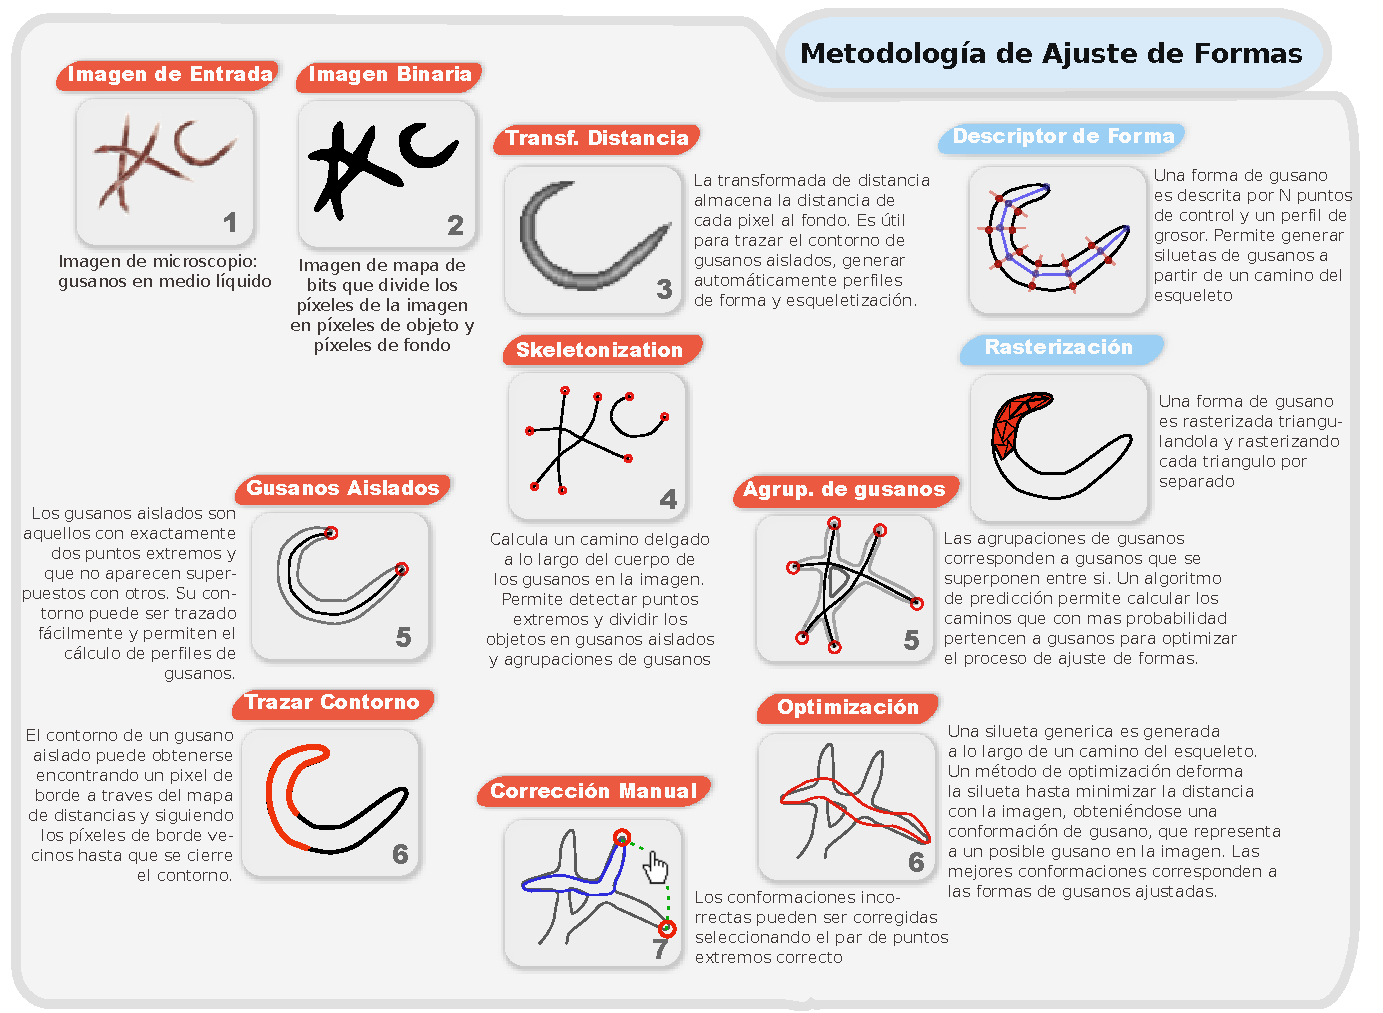
\includegraphics[scale=0.9,angle=270]{diagrams/design.pdf}
 \caption{Graphical description of the solution methodology for the shape detection
 of \emph{C.elegans} worms in digital images}
\label{fig:methsol}
\end{figure}

Given the input image, the first step is to separate the pixels belonging to the object
of study from the rest of the image pixels. A thresholding algorithm is then used to
obtain a binary image that separates worm pixels from background pixels. Usually some
noise is obtained after the thresholding process, but it is ignored in further processing.
This corresponds to an initial segmentation of the input. Once one have a binary image, a
distance map can be obtained in which each pixel represents the distance to the 
nearest background pixel, as explained in \cite{dtresearch}. The distance transformation
makes possible to identify the contour pixels in the binary image, which makes it a fundamental
tool for the automatic generation of a shape descriptor, contour tracing on isolated worms 
and optimization of the skeletonization algorithm, among others. Having the image 
separated in object pixels and background pixels, the image can be segmented to separate
the worms. \\

The image worms have been distinguished into two groups: \emph{isolated worms}
and \emph{worm clusters} (see Sec.\ref{sec:reasoning}). A way to differentiate the image worms
is to count the number of endpoints of every object (as defined after the binary transform).
An object with exactly two endpoints would correspond to an \emph{isolated worm} while
more than two points indicate the presence of overlapping worms, thus a \emph{worm cluster}.
At the same time a path from one endpoint of a worm to another is needed to match
the shape, due to the need of placing the matcher shape near to the matching shape, which
is a usual approach for shape matching, as covered in Sec. \ref{sec:shapefitting} and
Sec. \ref{sec:reasoning}. Having said this, a process of skeletonization would provide a simple
way to recognize endpoints as well as an approximated connected medial path between the
endpoints of the image objects. After this process, the image will be segmented into 
many different subareas of the images corresponding to both clusters and \emph{isolated
worms}. Each type of worm group is processed in a different way in order to match
the shape.\\

\subsubsection*{Isolated Worms}
The \emph{isolated worms} shape contour can be traced easily by selecting a border pixel
(indicated in the distance map) and following the neighboring contour pixels until the
initial pixel is reached back again. Then the whole shape can be rasterized by 
triangulating it through the \emph{ear clipping triangulation method} and then rasterizing
each triangle separately.This provides all the pixels belonging to the shape, 
\emph{i.e.} a match.
The nearly perfect match that can be obtained from the \emph{isolated worms} makes 
possible to calculate a worm profile from the currently analyzed worms in order to
generate an accurate shape descriptor (this is explained thoroughly in 
Sec. \ref{sec:metshapedescriptor}).

\subsubsection*{Worm Clusters}
To match the shape of the worms present in a \emph{worm cluster}, first the number of 
worms in the cluster is determined (follows from the number of
endpoints), then the best match between pairs of endpoints is found. Given a pair of 
endpoints, the path between them is calculated. Then a matcher worm shape is generated
from the shape descriptor, selecting a given number of control points in the path.
Afterwards an energy minimization process is performed that varies the angles between the 
straight lines that connect the control points (generating different shape representations),
until the best match is found. Finally the contour of the shape descriptor is slightly 
modified by finding the closest contour segments (or a lower value in the distance map)
to the contour points, in order to adapt the generic shape silhouette to 
the matching object. 

This process is repeated for every feasible worm path that can be found starting from
every endpoint, thus obtaining all the different worm conformations in the image.
Then an assignation algorithm would select the best set of conformations that maximizes
the number of covered endpoints and minimizes the total energy value. 
Since the total energy is the sum of energies of each worm, speed can be improved further 
by branch and bound.\\
A path guessing algorithm can be used to find the most likely path 
starting from a given endpoint. The conformation resulting from 
optimizing this path could be favored over the others in order to make
it more probable to be selected.\\

In the following sections, each of the subprocesses involved in the solution
methodology are explained, covering their need and usefulness as
well as the followed implementation approach.

% ADD THE MANUAL MODIFICATION OF THE RESULTS
  

\subsection{Thresholding}
\label{sec:metthres}

Since the main purpose of this study is to fit the shape of \emph{C.elegans} worms on digital
images, it is useful to differentiate these from the rest of the image in order to perform a more 
accurate analysis. The shape of the worms
can be characterized as objects and the rest of the image as background. More precisely
the image pixels can be separated into two groups: object pixels, that are all of those
that belong to a worm shape and background pixels, that are all the remaining ones.\\

Given this theoretical characterization, a thresholding filter would come to be a useful tool 
to locate the objects of study in the digital representation and to discard unnecessary 
information, obtaining a binary image from the original one. A binary image would then provide
an initial segmentation of the processed image, being as well a key element to obtain
a distance transformation, as explained in Sec. \ref{sec:metdt}.

\subsubsection{Implementation}
\label{sec:thresimp}
There are four thresholding filters for 2D images implemented on \emph{Endrov}, these are: 
\emph{Fukunaga}, \emph{Max entropy}, \emph{Otsu} and \emph{Percentile}, that cover the 
histogram and entropy-based thresholding methods categories as defined in Sec.\ref{sec:thresholding}.
Considering that the implemented methods are sufficiently different and given the transparency
of \emph{C.elegans} worms, it is hard to determine theoretically which would be the most appropriate 
thresholding method to obtain an accurate binary image from the study data-set. In order 
to select a thresholding method a series of experiments where performed tweaking the parameters
for the different mentioned methods.
The selected method was \emph{Percentile Threshold 2D} since is the easiest to tune manually and the 
one that calculated the best binary counterpart, given the characteristics of the images in the
data-set.

Figure \ref{fig:wormthres} shows a binary image obtained after applying
the \emph{Percentile Threshold 2D} method with a percentile value of $0.074$

\begin{figure}[h t b p ! H]
  \centering
  \subfloat[Original image]{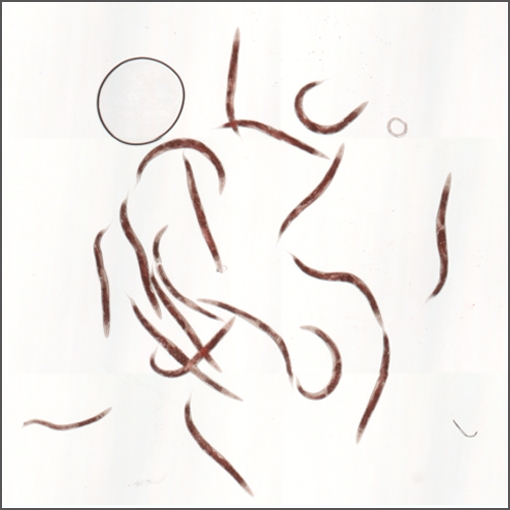
\includegraphics[width=0.45\textwidth]{original.png}}
\qquad
  \subfloat[Percentile Threshold. Value=0.074]{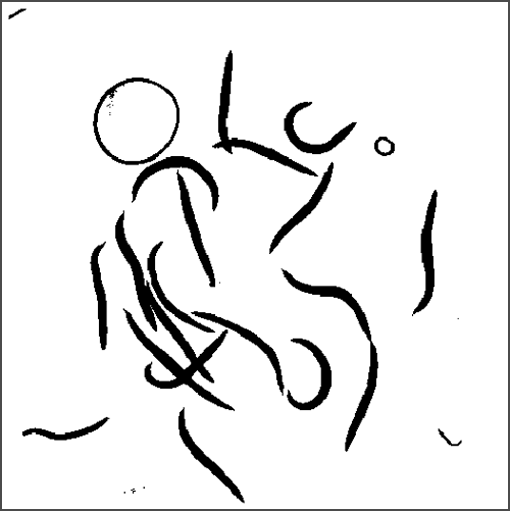
\includegraphics[width=0.45\textwidth]{thres/worms}}
\caption{Worms in liquid media. Original image and binary image obtained through
Percentile Thresholding with a percentile value of 0.074}
  \label{fig:wormthres}
\end{figure}

\subsection{Distance transformation}
\label{sec:metdt}

In this shape fitting approach for \emph{C.elegans} worms the distance transformation
of the given image is used thoroughly for contour detection and different kinds of image 
segmentation procedures. Specifically the distance map allows to detect and follow
the exact contour of isolated worms (Sec. \ref{sec:metiso}), 
is useful in the shape profile generation (Sec. \ref{sec:metwormprof}), and essential in the heuristic
guessing of the more likely worm-paths in \emph{worm clusters} 
(Sec. \ref{sec:pathguessing}).
It also improves the performance of the iterative thinning algorithm designed by 
\emph{Zhang and Suen} \cite{thinning} as it is described on Sec. \ref{sec:metsk}

\subsubsection{Implementation}
\label{sec:dtimp}

 As stated in \cite[p.196]{fastdt} the algorithms of distance transformation can be categorized into two classes: one is the iterative 
 method which is efficient in a cellular array computer since all the pixels at each iteration can be processed in parallel, and the other 
is sequential (or recursive) method which is suited for a conventional computer by
 avoiding iterations to be independent of object size. 
Using the general machines that most people working in digital image processing
 have access to, sequential algorithms are often much more efficient than
 iterative ones. For this reason a sequential approach was chosen to calculate the
distance transformation of the input images. Particularly the two-scans transformation
using 3x3 neighborhoods \cite{fastdt} which is both efficient and easy to implement.\\

In the mentioned paper a distance map calculation algorithm is described which consist
of only two scans of the image bitmap, one left to right - top to bottom, and another
right to left - bottom to top, with one operation per pixel. This makes the complexity
of the algorithm $\mathcal{O}(N)$ where $N$ is the size of the image array.
In \cite[p.197]{fastdt} a pseudo-code for \emph{Chessboard} and 
\emph{Manhattan or city-block} distances is given, while in \cite[p.198]{fastdt} the 
definition is extended to improve the efficiency of the calculations needed to 
generate a distance map using \emph{Euclidean} distances.
The two-scans algorithm was implemented using the three different distance metrics
mentioned before. This allows a wider analysis on the behavior and accuracy of the shape 
fitting process from one metric to another,``The city block or chessboard distance
measures are sensitive to the rotations of an object, but the Euclidean distance
measure is rotation invariant. However, its square root operation is costly...''
\cite[p.332]{eucskeleton}. Given the straight-like shape of worms and the different levels
of accuracy of the distance metrics it is hard to tell at first sight which would be 
the most adequate to use, so it had to be determined experimentally.
The figure \ref{fig:distance} shows the binary image and three distance maps obtained 
from a single worm image.

\begin{figure}[h t b p ! H]
  \centering
  \subfloat[Binary Image]{\label{fig:manh}
\includegraphics[width=0.45\textwidth]{dt/binary}}
\qquad
  \subfloat[Manhattan metric]{\label{fig:manh}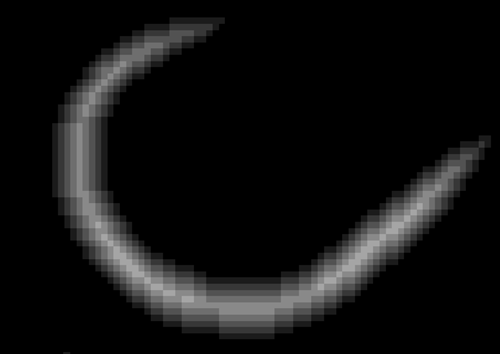
\includegraphics[width=0.45\textwidth]{dt/manhattandt}}
\qquad                
  \subfloat[Chessboard metric]{\label{fig:chess}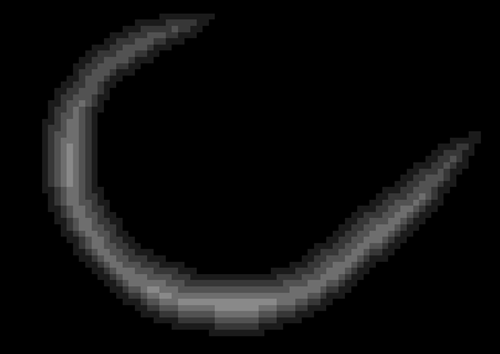
\includegraphics[width=0.45\textwidth]{dt/chessboarddt}}
\qquad
  \subfloat[Euclidean metric]{\label{fig:mouse}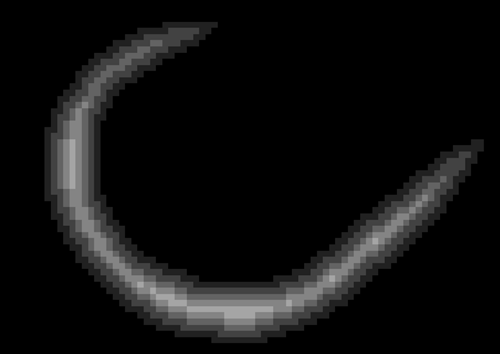
\includegraphics[width=0.45\textwidth]{dt/euclideandt}}
  \caption{Binary Image and Three Distance Transformation metrics from a single worm image}
  \label{fig:distance}
\end{figure}


\subsection{Worm Skeletonization}
\label{sec:metsk}

The skeletonization of the image corresponds to the process of obtaining a 
connected and thin (1-pixel width) medial axis that represents the worms in the 
image. This is a key process on the shape matching
approach followed in this work, as first mentioned on Sec. \ref{met:description}.
It makes possible to identify the amount of worms in the input image, to separate them 
distinguishing between \emph{isolated worms} and \emph{worm clusters}, and to
obtain an approximated path between endpoints 
of worms (that tends to the medial axis), which is the main element of the 
matching optimization process (see Sec.\ref{sec:metsegmentation}). The skeleton
image would then be fundamental to determine the area of the image in which
the worms are located and give estimated paths along which the different
worms would be disposed. \\

\subsubsection{Implementation}
\label{sec:skeletonimp}

For the purpose of this work the skeletonization algorithm to be selected must
ensure the connectivity of the skeleton points, \emph{i.e.} every skeleton point
must be connected to at least another skeleton point belonging to the same
skeleton. Also the skeleton connection must not be thicker than 1-pixel, this means that
when tracing a sequential path in the skeleton and being situated in a given skeleton 
point there must be only one neighbor skeleton point that can be selected to continue
the path direction, while remaining on the track of the skeleton of the same worm.\\

Provided that a distance map have been already calculated when the skeletonization 
process is carried out, an efficient approach would be to use a distance transform
based technique. Different methods consisting in finding ridge points on the distance
maps and then connect them have been covered in \cite{maxima,euclideancentre,ridgedt}.
The approach in \cite{maxima} was followed as a first attempt to calculate a thin
skeleton with a low time cost. This algorithm defines the ridge points as such pixels
that have the greatest numerical value among its 3x3 neighborhood (bitmap image) in the 
distance map. After finding the ridge points a \emph{up-hill} reconnection is performed, 
followed by a \emph{down-hill} connection for missing points. The study covered in \cite{maxima}
states that this approach makes possible to find successfully a connected 1-pixel-thin skeleton,
which was actually the case for \emph{isolated worms} or those which do not
overlap with other worms. Nevertheless for \emph{worm clusters} the obtained skeletons
were usually disconnected, thicker than 1-pixel and not accurate. Although the approach
seemed appropriate in theory, the costful reconnecting operations and the inaccurate
skeletons obtained for \emph{worm clusters} gave rise to the need for a different
approach.\\

Given the long, thin and cylindrical shape of the worms in general, a thinning algorithm
approach that reduces the different layers by removing pixels that should not 
belong to the skeleton was then taken into account. In \cite{thinning} an iterative and 
parallel thinning algorithm is presented, that consist in two sub-iterations per main 
iteration aimed at deleting the south-east boundary points and north-west boundary points 
respectively. The study is aimed at parallel computers so the different operations
in each pixel can be performed at the same time, improving the performance. In order
to avoid the requirement of using a parallel computer without losing the time performance 
improvement, the distance map was used to discard unnecessary pixel checking (those
belonging to inner layers). Thus in each iteration only the pixels belonging to the
currently selected shape layer are taking into account. The layers are defined by the
distance map value of its pixels. The first layer corresponds to a distance value
of one ($1$), the next to a distance value of two ($2$) and so on. This is presented in
algorithm \ref{thinninalg}.\\

\begin{algorithm}                     
\caption{Calculate shape skeleton}         
\label{thinninalg}                    
\begin{algorithmic}                   
\STATE $shapePts \leftarrow getBinaryObjectPixels()$
\STATE $dtImage \leftarrow getImageDistanceMap()$
\STATE $contourIndex \leftarrow 1$
\STATE $makeThinner = True$

\WHILE{$makeThinner$}

\STATE \COMMENT{remove south-east boundary points and the north-west 
corner point}
\FOR{$pixel$ in $shapePts$}
\IF{$dtImage(pixel) > contourIndex$}
\STATE \COMMENT{skip iteration}
\ELSE
\STATE $pixelRemove \leftarrow southEastCondition(pixel)$
\IF{$pixelRemove$}
\STATE $shapePts.remove(pixel)$
\STATE $makeThinner \leftarrow True$
\ENDIF

\ENDIF
\ENDFOR

\STATE \COMMENT{remove the north-west boundary points and the
		south-east corner points}
\FOR{$pixel$ in $shapePts$}
\IF{$dtImage(pixel) > contourIndex$}
\STATE \COMMENT{skip iteration}
\ELSE
\STATE $pixelRemove \leftarrow northWestCondition(pixel)$
\IF{$pixelRemove$}
\STATE $shapePts.remove(pixel)$
\STATE $makeThinner \leftarrow True$
\ENDIF
\ENDIF
\ENDFOR
\ENDWHILE
\STATE 
\RETURN{$shapePts$}

\end{algorithmic}
\end{algorithm}

The algorithm deals well with overlapping worms by constructing a path that is very close
from the shapes medial axis, and results in a totally connected 1-pixel width skeleton.
In fig. \ref{fig:skeleton} the skeleton of a sample image is shown. Every worm in the 
image that was previously identified in the binary image obtaining process 
(see \ref{sec:metthres}) is successfully \emph{skeletonized}.

\begin{figure}[h t b p ! H]
 \centering
   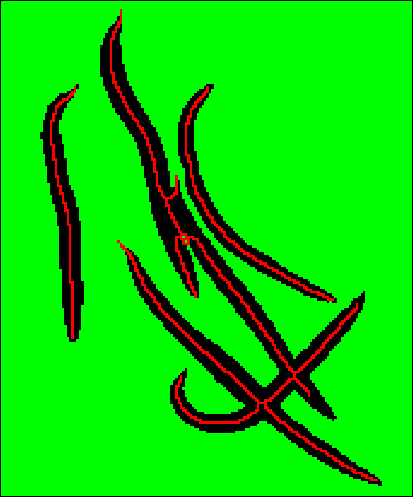
\includegraphics[scale=0.75]{skeleton/skeleton.png}
 \caption{Skeleton obtained through iterative thinning over a worm binary image}
\label{fig:skeleton}
\end{figure} 


\subsection{Worm Segmentation}
\label{sec:metsegmentation}

Since the goal is to match the shape of individual worms,
it is necessary to locate them in the image and then separate them 
as much as possible, \emph{i.e.} to segment the image.
This allows to improve the efficiency and accuracy of the 
shape fitting process, while reducing the matching area and thus the amount of 
different combinations that must be taken into account. After the process of 
\emph{skeletonization}, a set of paths are obtained 
between endpoints of worms (the objects of study), in some cases overlapping. 
By identifying the worm endpoints and tracing the paths that connect them together,
the different groups of paths can be separated, thus segmenting the image.
As explained in Sec. \ref{sec:metsk} and Sec. \ref{sec:reasoning}, the different groups
of paths can be distinguished, in correspondence to the objects they represent,
by \emph{isolated worms} and \emph{worm clusters}. Then the shape fitting process
of the whole image would consist of matching and fitting the worms present in each of
the obtained sub-images separately.\\

Another process of segmentation that is performed is the identification of single
worms paths, in both \emph{isolated} and \emph{cluster} worms. For \emph{isolated worms}
the path that determines its medial axis is used for two different processes. 
First to find the surrounding contour to
fit its shape (see Sec. \ref{sec:metiso}). And second, to generate a profile that 
would define a general representation of the worms in the image through a shape
descriptor, as is explained in Sec. \ref{sec:metwormprof}.
On the other hand, for \emph{worm clusters}, feasible worm paths must be found between endpoints. 
If a path exist between a pair of endpoints then a valid worm conformation between them will
be generated through the optimization process.
These paths are chosen among all the technically possible paths between endpoints, and by
a more sophisticated path guessing algorithm that will be described below in the
implementation section.


\subsubsection*{Worm Endpoints}
\label{sec:wend}
The skeleton calculation returns an image 
containing 1-pixel-width groups of curves or paths.
The pixels that are connected with 
two or more other pixels (neighbors) are \emph{body-pixels}, which belong 
to the path and are not endpoints. On the other hand those that are connected with 
only one other pixel are endpoints, thus each one could belong to the extreme of a
worm. It is important to consider that since the thinning algorithm used to obtain
the skeleton (covered in Sec. \ref{sec:skeletonimp}) consists in removing the shape
layers until finding pixels that are not surrounded, the endpoints found in the
skeleton will not necessarily correspond to worm endpoints.\\

In order to find the pixels that are actually worm endpoints a skeleton expanding process
is performed that aims to stretch the skeleton path up to a contour point that 
would come to be the worm endpoint. The skeleton expanding algorithm uses the definition
of \emph{directional neighborhood} stated in \cite[p.334]{maxima}, where given 
a pixel $P$ in the bitmap, a \emph{directional neighborhood} $D$ of $P$ is 
conformed by those pixels that belong to the \emph{8-neighborhood} of $P$ and that
are located within $\pm$ $45^{\circ}$ slope changes from the current medial axis 
orientation of $P$. In fig. \ref{fig:directional} three examples of directional
neighbors are presented. The algorithm consist in following the best directional path
starting in every endpoint and expanding the skeleton until a contour pixel is found.
 
\begin{figure}[h t b p ! H]
 \centering
   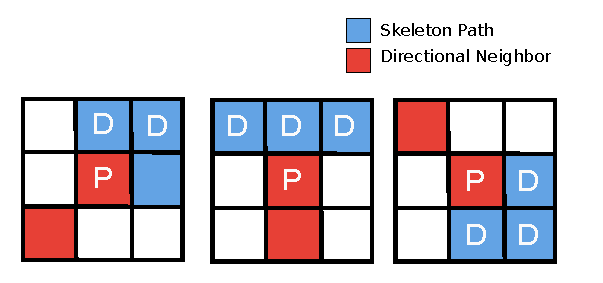
\includegraphics[scale=1]{skeleton/directional.pdf}
 \caption{Three different directional neighborhoods}
 \label{fig:directional}
\end{figure}

The expanding algorithm can be summarized in the following steps:
\begin{itemize}
\item Select an endpoint
\item Find the previous skeleton point and calculate the directional neighborhood
\item Select the directional neighbor with the lowest distance transformation pixel,
  and mark it as skeleton pixel.
\item If the neighbor is not a contour point repeat the process.
\end{itemize}

A filtering process is done to remove incorrect object pixels, that consists in
removing skeletons that have a size (number of pixels) lower than a small 
threshold. This allows to remove some slightly noisy regions and incorrect endpoints.
Once the skeleton is successfully expanded, the endpoints of the skeleton are considered
worm endpoints. 
It must also be considered that some worm endpoints cannot be detected following this 
process, particularly in crowded images where there is a big chance that the
overlaps ``hide'' the endpoints. Nonetheless, a manual process can 
be carried out to add the missing endpoints, as explained in Sec. \ref{sec:manualproc}.



\subsubsection*{Group segmentation}

Having detected every worm endpoint, the image can be segmented by determining
the endpoints that are bound together through a skeleton path, \emph{i.e.} finding 
the different \emph{isolated worms} and \emph{worm clusters}.
As previously explained, the overlapping worms in the image are bound together
as one object in the binary image obtaining process, so then in the skeletonization
process the endpoints belonging to \emph{worm clusters} are bound together as well,
through a skeleton path.
Based on the previous reasoning an algorithm was designed that detects the endpoints 
that are bound together through the path that links them, separating the 
linked paths into different groups. Those paths that link together exactly two
endpoints represent \emph{isolated worms} while a different number of endpoints
correspond to \emph{worm clusters}.
This method is described in algorithm \ref{groupsegment}. The algorithm consist of
basically following every different
possible path starting on an endpoint until all the endpoints of a group have been 
reached. 

\begin{algorithm}                     
\caption{Calculate shape skeleton}         
\label{groupsegment}                    
\begin{algorithmic}                   

\STATE $endPtList \leftarrow$ list of endpoints
\STATE $clusterIndex \leftarrow$ 0
\FOR{$endpoint$ in $endPtList$}
\IF{$endpoint.wasVisited()$}
\STATE \COMMENT{skip iteration}
\ELSE
\STATE $clusterIndex +=1$
\STATE $followPath(endpoint,clusterIndex)$
\ENDIF
\ENDFOR
\end{algorithmic}
\end{algorithm}

\begin{algorithm}                     
\caption{Follow Path algorithm ( $followPath(currentPoint,clusterCount)$ )}         
\begin{algorithmic}                   

\REQUIRE $currentPoint$
\REQUIRE $clusterCounter$

\IF{not $currentPoint.isSkeletonPoint()$}
\RETURN 
\ELSE
\STATE $addToCluster(endpoint,clusterIndex)$
\ENDIF

\STATE \COMMENT{continue tracing path}
\IF{$currentPoint.isEndPoint()$}
\STATE $markEndPointAsVisited(currentPoint)$
\ENDIF
\STATE $neighbors \leftarrow getNeighborhood()$
\FOR{$n$ in $neighbors$}
\STATE $followPath(endPoint,clusterCounter)$
\ENDFOR

\end{algorithmic}
\end{algorithm}


\subsubsection*{Path guessing}
\label{sec:pathguessing}

The \emph{worm clusters} found through segmentation are defined by a set of endpoints
that are all connected through \emph{skeleton} paths, however the pair of endpoints
belonging to each worm in the image and an accurate skeleton path that
connects them is still unknown. The optimization algorithm, covered in \ref{sec:metfit},
performs a shape manipulation process to match the worms in the image given two endpoints
and the path that connects them. When the right skeleton paths are unknown the algorithm
tries every possible combination returning the best match as possible, with the 
consequent overhead in performance time . In order to improve the time efficiency of the 
algorithm as well as the accuracy of the matching (particularly avoiding incorrect
endpoints bounding), a path guessing algorithm was designed that performs a heuristic
guessing of the most-likely path between endpoints.\\

The algorithm is based on the idea of avoiding paths that continue unnatural conformations
of the worms shape. This means that given $S$ last steps in the skeleton tracing, the
next step $S+1$ will tend to follow the direction that was being followed, thus
avoiding unnatural bendings or abrupt changes in the shape. An important issue when 
following the most common direction in the last $S$ steps is that in some cases
the path tracing will tend to avoid \emph{path bifurcations}. 
A \emph{path bifurcation} occurs when there is more than one neighbor pixel that can be 
followed next, thus dividing the path in two or more different paths.\\

In order to make the path tracing tend to reach path bifurcations and then decide the best
path to take, a heuristic function was designed that consists of the value of the neighbor pixel
in distance transformation multiplied by a variable factor.
Then the selection of the next pixel to follow is based on two main values:
the amount of time that the neighbor direction has been taken in the last $S$ steps and
the distance map value of the pixel. This can be expressed as below:

$$Next(p) = \max_{n \in neighbors(p)} (dirValue(direction(p,n),S) + dt(n)*hfactor)$$

where $p$ is the current path pixel, $dirValue$ returns the amount of times that the 
direction of the neighbor pixel $p$ have been taken in the last $S$ steps, $dt$ is the 
distance map and $hfactor$ is a heuristic factor that controls the influence of the
distance map.

In order to cover the issue mentioned in Sec.\ref{sec:wend}, that some endpoints could
be hidden because of the overlapping, the number of pixels that have been added
to a tracing path are counted, so when it is not possible to reach any other endpoint,
an extra endpoint is created after $wormLength$ steps. 
The $wormLength$ is an estimated value that is calculated
as the mean of the length of the \emph{isolated worms} in the image. This process
attempts to identify worms that otherwise would be discarded because of the absence
of endpoints. Algorithm \ref{guess} presents a pseudo-code for the path
guessing approach.

\begin{algorithm}                     
\caption{Pseudo-code algorithm for path guessing between endpoints}         
\label{guess}                    
\begin{algorithmic}                   

\STATE $endPtList \leftarrow$ list of endpoints
\STATE $wc \leftarrow$ paths and endpoint in worm cluster 
\STATE $length \leftarrow$ worm estimated length multiplied by a scaling factor
\FOR{$endPoint$ in $endPtList$}
\IF{$alreadyReached(endPoint)$}
\STATE \COMMENT{skip iteration}
\ENDIF
\STATE{$markAsReached(endPoint)$}

\STATE $path \leftarrow$ empty list

\STATE $reachedEndPoint \leftarrow False$
\STATE $currentPixel \leftarrow endPoint$
\WHILE{$not(reachedPoint)$ and $size(path)<length$}
\STATE $currentPixel \leftarrow getBestNeighbor(currentPixel)$
\STATE $updateDirectionsArray(direction(currentPixel))$
\STATE $path.add(currentPixel)$
\IF{$isEndPoint(currentPixel)$}
\STATE $reachedEndPoint \leftarrow True$
\ENDIF
\ENDWHILE 

\IF{$not(reachedEndPoint)$}
\IF{number Of Reachable Endpoints $= 0$}
\STATE $createEndPoint(currentPixel)$
\STATE $path.add(currentPixel)$
\ELSE
\STATE \COMMENT{Select a path to reachable endpoint}
\ENDIF
\ENDIF
\ENDFOR

\end{algorithmic}
\end{algorithm}

\subsection{Worm Shape Descriptor}
\label{sec:metshapedescriptor}

As first mentioned on Sec. \ref{met:description} the selected methodology approach 
to match \emph{C.elegans} worms is based on the manipulation of 
worm shapes generated from a shape descriptor.
Worm shapes can be described in geometrical terms as long, thin and cylindrical 
objects. Given that the process of skeletonization and image segmentation allow
to obtain \emph{thin} paths between pairs of endpoints that correspond to worm 
extreme points, a shape descriptor would permit to construct a shape around this
medial axis that would work as a starting point for the optimization algorithm. \\

A shape descriptor was then designed based on the idea of generating a representative
worm shape around the medial axis. The descriptor consists of two 
elements: control points and a shape profile (worm profile). The control points are
a set of $N$ equidistant points along the worm medial axis, both endpoints included.
Each control point has associated a \emph{thickness} value that represents the
radius of a circle with the control point as center. Then by selecting two points
in opposite directions of the thickness circle for every control point, and joining
these points together through a smooth curve, a contour line is obtained that traces
the silhouette of a worm shape, as shown in fig. \ref{fig:descriptor}. 
The set of \emph{thickness} values that are associated to each control point
is called a shape profile (worm profile for this study).

\begin{figure}[h t b p ! H]
 \centering
   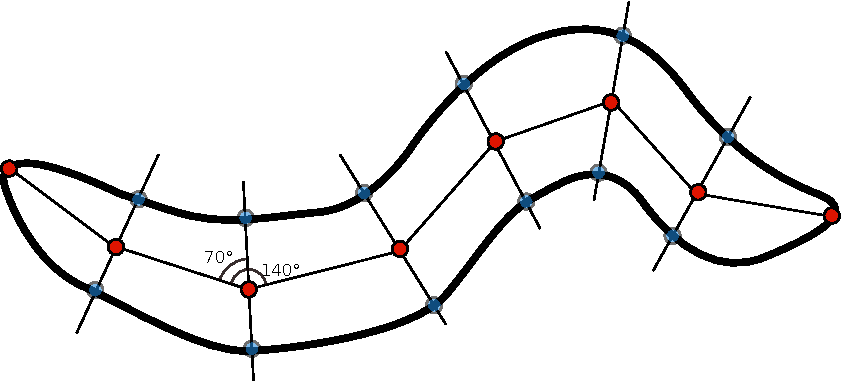
\includegraphics[scale=1]{descriptor/descriptor-vector.pdf}
 \caption{Construction of a worm shape based on shape descriptor}
 \label{fig:descriptor}
\end{figure}

In order to obtain a contour that accurately represents the worm shape along the 
medial axis, the choice of the opposite points in the \emph{thickness} circles 
must take into account the \emph{skeleton} bendings.
Since the shape is constructed following the \emph{thickness} of control points,
the bendings in the generated shape occur at each of these ones, and can then be 
calculated as the angle between the straight lines that connect the control points.
The bisection of any angle provides a straight line that divides it
into two equal portions, measuring the bending variation at each control point.
Then selecting the two points at a respective \emph{thickness} distance, from every control
point, following the bisection line in opposite directions provides a set of points
that joined together with a smooth curve will give a worm shape contour.\\

Generating a smooth curve around the control points improves the accuracy of the shape
description, compared to tracing straight lines
between the contour points. At the same time it allows to obtain a good representation
of the shape with a considerably smaller number of control points. The smooth curve
is obtained by calculating the cardinal spline (covered in Sec. \ref{sec:splines}) given the
contour points. A cardinal spline is a function that describes a smooth curve that
passes over all the points of a set, given a starting and ending point. In this case
the starting and ending points are the same, so the described contour is closed.\\

The worm profile for a set of control points can be both manually set or automatically
calculated from the \emph{isolated worms} as explained in the section below.

\subsubsection{Automatic Profile generation}
\label{sec:metwormprof}

The shape of \emph{isolated worms} identified in the image can be accurately matched
by following the contour points in their respective distance map, as explained 
in Sec. \ref{sec:metiso}. Given a set of matched shapes for \emph{isolated worms}, and
the initially detected skeleton, a worm profile (as described previously) can be 
generated by measuring the \emph{thickness} of every control point and finding the mean
among these.\\

In order to measure the thickness for every control point, a set of
$N$ equidistant points is generated that cover the skeleton of the \emph{isolated worm}.
Then as described in the previous section, the bisectors of the angles between the 
straight lines connecting the control points are calculated. Starting from every control
point, the bisector line is ``walked'' until the pixel with the lowest distance map
value is found, a contour point in most of the cases. The operation is repeated for every 
control point bisector in both opposite directions. The Euclidean distance from a control
point to each found pixel is calculated, and its average is recorded. Repeating this process
with every \emph{isolated worm} generates a set of \emph{thickness profiles}, one for each
\emph{isolated worm}. Then a general worm profile is calculated by finding the mean between
the thickness values for every control point in each \emph{thickness profile}. In order 
to generate an accurate profile, that avoids oversized (or downsized) worms and wrongly
detected \emph{isolated worms}, the $20\%$ higher and lower values are discarded when 
calculating the average. The \emph{thickness} value for
the endpoints, \emph{i.e.} the first and last point in the set of length $N$, is zero,
so one contour point is generated in the extremes instead of two.
Having done this a \emph{thickness profile} is obtained that represents the average 
radius distance for every control point to its closest contour pixel, making possible
to generate a generic worm shape around any skeleton defined by $N$ points. 

\subsection{Shape rasterization}
\label{sec:metrast}

The proposed matching approach is focused on minimizing the difference between generated
shapes and the shapes in the image. In order to do so the area covered by the matching shape
must be calculated.\\ 
Given a shape descriptor, a worm shape can be
constructed following a worm profile consisting of a worm silhouette defined by 
a b-spline curve. Given the contour of the worm shape, the area can be calculated and 
then rasterized in order to express it in image data terms.\\

The approach followed to achieve this consists of triangulating the space defined by the
closed contour of the shape and then rasterizing every triangle by separate. The
decomposition of a polygon into simple triangles whose vertices are only those of
the simple polygon is a classic problem in computer graphics. So, many solutions
has been proposed such as: Delaunay triangulation, minimun-weight triangulation and
the ear clipping method, among others. The ear clipping method was chosen because
of its capacity to triangulate concave polygons and its ease of implementation.
In order to convert the worm outline into a polygon, the spline curve that defines it 
is transformed into a discrete set of points. Each successive point is connected
by a straight line, defining the closed polygon. Then this polygon-like worm shape
is triangulated.\\

Every triangle defining the area is rasterized following the \emph{scan conversion algorithm}
explained in \cite{scanconversion}. The algorithm consists in tracing horizontal lines 
between the edges of the triangle until the area is totally covered.\\

This process calculates a set of pixels that constitute the area of the shape. Thus, 
the area and contour of the shape can be stored as manageable and displayable data.


\subsection{Profile-driven shape fitting}
\label{sec:metfit}

Once the initial processing of segmentation and worm skeletonization is performed, where 
information about the worms in the image is gathered, a shape matching process has to be 
carried out in order to detect the shape that corresponds to each worm, 
following the prior information. The matching process is different for
\emph{isolated worms} and \emph{worm clusters}  
due to their nature. In this sections each process is explained and some 
implementations details are given.


\subsubsection{Isolated Worms shape fitting}
\label{sec:metiso}

At this point the information gathered about each \emph{isolated worm} consists in 
a 1-pixel skeleton path between exactly two endpoints. Since this process is carried
out after each endpoint is identified correctly, the area conformed by the object pixels
surrounding the skeleton will correspond to the exact shape of the \emph{isolated worm}.\\

In order to optimize the calculation of the worm area, the contour of the shape is first
traced and then the internal area is triangulated and rasterized following the process
explained in \ref{sec:metfit}. The contour is traced by finding the closest border-pixel
to any endpoint and then following the neighbor that is also a border-pixel. A
border-pixel is such that has a value of one (1) in the image distance map.
This makes possible to obtain the contour and area of the worm shape corresponding to each 
\emph{isolated worm} accurately.


\subsubsection{Worm Cluster shape fitting}
\label{sec:clusterfit}

The \emph{worm clusters} represent a more complicated shape matching scenario due to their
variable number of worms and the many different possible conformations that can be detected
on them. 
The  overlaps in \emph{worm clusters} makes difficult to differentiate the group of pixels
that belong to the area of one worm or another. A matching process must then be 
carried out that calculates the most likely worm conformation that starts from every
endpoint in order to obtain the set of conformations that best fit the whole 
\emph{worm cluster}.\\

A shape optimization matching approach was followed that consists of calculating all the 
worm conformations starting from any endpoint. A worm conformation is obtained by generating
a generic worm shape from a skeleton path and deforming that shape until the dissimilarity
between the generated shape and the binary image is minimum. Below, the main steps and 
features of the algorithm are described:

\begin{itemize}
\item For every endpoint the set of feasible skeleton paths starting from that pixel
  are calculated.
\item Given a skeleton path, a generic worm shape is constructed by generating a shape
descriptor following the worm profile of the image.
\item An optimization process deforms the generic worm shape until the dissimilarity
between the shape and the corresponding binary image is minimized. The optimized
shape corresponds to a feasible worm conformation.
\item Once all the possible conformations from every endpoint are calculated, a set of
conformations is selected that maximizes the number of endpoints covered and minimizes
the sum of the energy values. The selected conformations are the best automatic matches.
\end{itemize}

\subsubsection*{Shape deformation}

The calculated skeleton paths starting from a given endpoint are guesses of possible
worm skeletons. Since the deformed model is constructed over a skeleton path 
(that is close to the medial axis of the \emph{worm cluster}) the initially generated 
shape will always be close to a worm shape. Given this, just slight perturbations of
the generated shape would deform the model sufficiently to correct the deviation of the
skeleton from the actual medial axis, obtaining thus the most likely worm shape
over the given path.\\

The deformations are made over a shape descriptor, that is defined by a series of 
control points and constructed following a worm profile. In order to provide feasible
shapes and to limit the number of possible deformations, a deformation will consist
in the repositioning of a given control point. The number of different positions that a 
given control point can take is fixed and set along the bisection of the angle between
the lines that connect the previous, current and next control point. 
Following this, the set of deformations that can be performed from an initial shape 
can be calculated quickly and provides a great number of possible different conformations.\\

\subsubsection*{Energy Formulation}
 
The distance function must provide a measure of how far the deforming shape is from a worm in the image, 
\emph{i.e.} how well
the deforming shape fits. To measure the dissimilarity between a given worm shape and the
matching image, an energy formulation was followed, based on Active Contour Models,
\cite{snakes}, that consists of an external energy and an internal energy.\\

The external energy models how well the deformed model matches the data. Since the more
background pixels are covered the farther the model is from a worm in the \emph{worm cluster}, 
then a good measure for the external energy would be the proportion of background pixels in the 
area covered by the deformed model.Then, the more object pixels are covered the lower the 
external energy is. So, given a model $M$ and the functions $bg$ and $fg$  that measure
the amount of background and foreground pixels respectively, the external energy
can be defined as:

$$E_{ext}(M) = \frac{bg(M)}{bg(M)+fg(M)}$$

The measure is not considered just as the sum of background pixels
because the energy value will be vary to much, given the variability of the amount
of pixels covered by a worm shape.\\

The internal energy is the one that models the objects resistance to be deformed into
a shape that do not corresponds to the modeling class, \emph{e.g.} the worm class. 
This means that the internal energy resists to obtain not feasible worm
shapes after deformation. The internal energy for
snakes, as explained in \cite{snakes}, works as a smoothness constraint and is explicitly
formulated (usually in terms of first and second derivatives). As stated in \cite{bspline}, 
many problems arising from this formulation have been recognized in literature such as:
slow convergence speed, difficulty in determining the weights associated with the 
smoothness constraint, high order derivatives on discrete curves may not be accurate
in noisy environments.\\
However, in the approach proposed in this work, every shape is generated from a worm 
profile following a shape descriptor,so every deformed shape will still belong to the 
worm class. Thus it is not necessary to include the internal energy in the 
formulation.

\subsubsection*{Matching Optimization}

The optimization process consists in obtaining the most likely worm shape that can be
obtained by deforming a shape constructed over a skeleton path, known as a 
worm conformation. Given how quickly the different deformations can be computed,
a local-search optimization approach is followed. The process consists in obtaining the
best individual in the neighborhood that improves the energy function, until is 
minimized. The neighborhood is calculated in the following way:
For a given shape, four (4) different deformations are calculated for control point.
The possible deformations or new positions are the
next and second next position in north and south direction, \emph{i.e. }the two opposites
directions of the bisection of the control point.
There are then $N*4$ different possible deformations (neighbors) for a given shape,
where $N$ is the number of control points.\\ 
Then a neighborhood consists of mild and slightly stronger deformations of a given
worm shape for any control point.\\ Since the focus is to obtain the most accurate worm 
shape for a given skeleton, the
first and last control points, that correspond to the worm endpoints, are fixed.\\

Once the best shape is obtained a contour fixing process is carried out, that
consists in the expansion or contraction of the contours of the shape in order to adapt
to the actual worm in the image. This is required since the optimized shape is built 
following a worm profile, that just represents the shape of the worms in the image 
generically. In this process the extremes constructed from the control points are pushed
to contour points following the distance map, either expanding or contracting. While
expanding or contracting, every considered new possible position must have either the 
same or lower distance map value. A better point must be found after a fixed number
of steps, otherwise is discarded. This is done to avoid too big and strange deformations.

\subsubsection*{Conformations Assignment}

After the optimization process is performed, a subset of all the possible calculated 
conformations for \emph{worm cluster} must be selected, thus obtaining the image
worms match. The selected subset must maximize the number of endpoints covered and 
minimize the sum of energies of the conformations.\\
Any given endpoint may belong to at most one conformation. So, to any endpoint
there corresponds one and only one other endpoint. Therefore, the optimal subset of
conformations would be the minimal assignment between the sets of endpoints.\\
This can be obtained by solving the non-bipartite graph assignation problem. However,
given the implementation complexity (and possible performance overhead) of this algorithm,
another greedy algorithm was designed. The implemented algorithm consists in a iterative 
greedy solution. The algorithm is applied for the subclusters of \emph{worm clusters}. 
This subclusters comprehend just the endpoints that are connected 
by feasible paths. The endpoints belonging to a given subcluster will be called 
conflicting endpoints.\\

The algorithm consists in the following:
Given $N$ conflicting endpoints a $NxN$ table is constructed indicating the cost
of the best conformation that connects a endpoint with another. Then for a given 
starting row endpoint the lowest value is selected, and an assignment is made
between the row endpoint and the column endpoint (row and column are always different).
All the conformations starting from the row and column point are deleted.
Then, among the remaining rows, the one with the lowest value among the possible matches
is selected. The process is repeated after all the possible endpoints are assigned, thus
finding a solution. Once a solution is found, it is stored, the table is reconstructed and
the process is repeated starting from a different row, until all the rows have been taken
as starters. From all the gathered solutions, the one with the higher number of endpoints
covered and minimum total energy value is selected as the subcluster assignment.

\subsection{Manual Adjustment}
\label{sec:manualproc}

A process of manual adjustment can be performed by the user to improve the shape fitting
accuracy, such as adding missing endpoints or fixing wrong worm conformations. Below
both mentioned manual processes are explained. 

\subsubsection{Endpoint operations}
\label{sec:endpointop}

Worm endpoints are detected by first identifying extremes in the worm
skeleton. However when the extreme of a given worm in an image overlaps with 
another worm shape, the shapes become continuous so the shape skeleton will be generated 
as a continuous path. Thus, the extreme point will be missing and the endpoint will not be 
detected. Since the solution methodology is centered on finding paths between endpoints and 
then determining the most likely worm paths, having missing endpoints could affect 
the matching accuracy.\\

Worm endpoints are simple to detect for a human being, once had the skeleton of the 
a worm cluster, so the missing endpoints could be added quickly by following a manual
process. This process consists in looking at the extreme of worms and adding an 
extreme point when missing. Since by definition an endpoint is the extreme of a worm path,
it must have one and only one neighbor belonging to the skeleton. When an added extreme
point has more than one skeleton neighbor, the user would have to select the extra
neighbor pixel for deletion.
In summary the user can add the missing endpoints by selecting the missing pixel
and perhaps selecting some neighbors as well if it is necessary to disconnect. 

\subsubsection{Match Fixing}
\label{sec:matchfix}

After the optimization process is completed for the whole image, a set of 
worm conformations is given that corresponds to the best match assignation.
For some images there are worms that are not matched correctly, so 
conformations are given between incorrect pair of endpoints. 
Since in the optimization process all the possible conformations are calculated
between pair of endpoints, the wrong assignation could be fixed manually. A user
can recognize easily which conformations are incorrect, as well as quickly 
identify the endpoint that corresponds to any other endpoint. Then, by selecting 
the correct pair of endpoints, the corresponding
conformation will be modified, thus obtaining a correct fitting.



